\documentclass{beamer}
\setbeamertemplate{footline}[frame number]

\usepackage{graphicx} % Required for inserting images
\usepackage{float}
\usepackage[section]{placeins}
\usepackage{subcaption}
\usepackage[labelfont=bf]{caption}
\usepackage[backend=biber, sorting=none,  style=numeric-comp]{biblatex}
\usepackage{amssymb}
\usepackage{amsmath}
\usepackage{setspace}
\usepackage{hyperref}

\RequirePackage{silence}
\WarningFilter{latexfont}{Font shape `}

\usepackage{tikz}
\usetikzlibrary{arrows.meta}
\usetikzlibrary{positioning}

\DeclareMathAlphabet{\mathbbold}{U}{bbold}{m}{n}
\newcommand{\identity}{\mathbbold{1}}
\usepackage{mathtools}
\DeclarePairedDelimiter\abs{\lvert}{\rvert}
\DeclarePairedDelimiter\bra{\langle}{\rvert}
\DeclarePairedDelimiter\ket{\lvert}{\rangle}
\DeclarePairedDelimiter\expected{\langle}{\rangle}
\DeclarePairedDelimiterX\braket[2]{\langle}{\rangle}{#1\,\delimsize\vert\,\mathopen{}#2}

\title{\textbf{Non-Adiabatic Strategies for Quantum Optimisation Algorithms: Quantum Walk and Optimal State-Transfer}}

\pdfstringdefDisableCommands{%
  \def\\{}%
}
\author{ Chayapon Thunsetkul \\
	Advisor: Dr. Alejandra Beghelli
}

\date{\today}

\newcommand{\Nb}{N_{\text{best}}}
\newcommand{\Np}{N_{\text{pair}}}
\addbibresource{../project_report/references/merged.bib}
% \bibliographystyle{ieeetr}
\usepackage[table,HTML]{xcolor}
\definecolor{RED}{HTML}{d20f39}
\definecolor{PEACH}{HTML}{fe640b}
\definecolor{TEAL}{HTML}{179299}
\definecolor{PINK}{HTML}{ea76cb}
\definecolor{SKY}{HTML}{04a5e5}
\definecolor{BLUE}{HTML}{1e66f5}
\definecolor{BLACK}{HTML}{4c4f69}

\newcommand{\reddashed}{\tikz[baseline=-0.5ex]\draw[RED,dashed, line width = 1pt,font=\boldmath] (0,0) -- (0.5,0) node[midway]{ \scriptsize $\times$};}
\newcommand{\peachdashed}{\tikz[baseline=-0.5ex]\draw[PEACH,dashed, line width = 1pt,font=\boldmath] (0,0) -- (0.5,0) node[midway]{\scriptsize $\times$};}
\newcommand{\pinkdashed}{\tikz[baseline=-0.5ex]\draw[PINK,dashed, line width = 1pt,font=\boldmath] (0,0) -- (0.5,0) node[midway]{\scriptsize $\times$};}
\newcommand{\skydashed}{\tikz[baseline=-0.5ex]\draw[SKY,dashed, line width = 1pt,font=\boldmath] (0,0) -- (0.5,0) node[midway]{\scriptsize $\times$};}
\newcommand{\blackline}{\tikz[baseline=-0.5ex]\draw[BLACK,solid, line width = 1pt,font=\boldmath] (0,0) -- (0.5,0) node[midway]{\scriptsize $\times$};}
\newcommand{\blackdashed}{\tikz[baseline=-0.5ex]\draw[BLACK,dashed, line width = 1pt,font=\boldmath] (0,0) -- (0.5,0) node[midway]{\scriptsize $\times$};}
\title{
Using QAOA for Routing and Wavelength Assignment Optimisation in Optical Networks
}
\begin{document}
\frame{\titlepage}
\begin{frame}{Routing and Wavelength Assignment (RWA)}
    \begin{itemize}
        \item In wavelength division multiplexing (WDM) network, a connection between a source and a destination node is established by a lightpath.
        \item A lightpath is a set of links associated with a unique wavelength.
        \item A lightpath must \begin{enumerate}
                \item have all of its link using the same wavelength (wavelength continuity), and
                \item not use the same wavelength as another lightpath sharing same link(s).
            \end{enumerate}
        \item The task of assigning routes and wavelengths optimally is called the Routing and wavelength assignment (RWA) problem\cite{Birman515906}.

    \end{itemize}
\end{frame}
\begin{frame}{Motivation}
    \begin{itemize}
        \item The problem is NP-complete and exact solutions are intractable at large scales\cite{Chlamtac101539, Birman515906, Bala147477}.
        \item Classical heuristics (e.g.\ shortest-path first-fit) provide good but not necessarily optimal solutions\cite{Chlamtac101539, Birman515906, Bala147477, Subramaniam605312, Gibong497889, Karasan664267, Barry719747}.
        \item Quantum and quantum-inspired methods, have been investigated as potential alternatives\cite{Seker01022024, boev2023}.
        \item One of the main limitation of these quantum approaches is that hard constraint must be modelled as penalties in the cost function, yielding infeasible solution.
    \end{itemize}
\end{frame}

\begin{frame}{QAOA}{Quantum Approximate Optimisation Algorithm}
\begin{itemize}
    \item Given a cost function $f(x)$, define the \textit{problem Hamiltonian}:
\begin{align}
    \hat{H}_{P} \ket{\boldsymbol{x}} = f(\boldsymbol{x}) \ket{\boldsymbol{x}}. \label{eq:Hp}
\end{align} and another Hamiltonian called the \textit{mixer Hamiltonian} usually taken to be the transverse-field Hamiltonian:
\begin{align}
    \hat{H}_{m} = - \sum_{j} \hat{X}_{j}, \label{eq:Hm}
\end{align}
\item Define two parameterised unitaries: the \textit{phase operator}
    \begin{align}
        U_{P}(\gamma) = e^{-i \gamma \hat{H}_{P}} \label{eq:up}
    \end{align}
    and the \textit{Mixing operator:} \begin{align}
        U_{M}(\beta) = e^{-i \beta \hat{H}_{M}} \label{eq:um}
    \end{align}
\item Initial state: equal superposition $\ket{\psi_{i}} = \frac{1}{\sqrt{2^{n}}} \sum_{\boldsymbol{x}} \ket{\boldsymbol{x}}$
\end{itemize}
\end{frame}

\begin{frame}{QAOA}{circuit}
After $P$ alternating layers, the final state is
\begin{align}
    \ket{\boldsymbol\beta, \boldsymbol\gamma} &= \hat{U}_{M}(\beta_{P-1}) \hat{U}_{P}(\gamma_{P-1}) \cdots 
    \hat{U}_{M}(\beta_{0}) \hat{U}_{P}(\gamma_{0}) \ket{\psi_{i}}, \label{qaoa-equation}
\end{align}
\begin{figure}[H]
    \centering
    \includegraphics[width=\textwidth]{pictures/circdiagram.pdf}
    \caption{
        A $P$-layer QAOA circuit on $n$ qubits. Each layer applies a problem unitary 
    }
    \label{qaoa-circ}
\end{figure}
Objective: find parameters $(\boldsymbol{\beta}, \boldsymbol{\gamma})$ minimising
    \[
        \langle f \rangle = \bra{\boldsymbol\beta, \boldsymbol\gamma} H_{P} \ket{\boldsymbol\beta, \boldsymbol\gamma}.
    \]
\end{frame}

\begin{frame}{QAOA}{Quantum Alternating Operator Ansatz}
    \begin{itemize}
        \item Consider a problem where we only want to find a solution that belongs to a set of \textit{feasible} solution which is a (proper) subset of the set of all solutions.
        \item Using the tranverse-field Hamiltonian does not preserve the feasible subspace.
        \item The extension of the original QAOA introduced in \cite{Hadfield_2019-Quantum-Alternating-Operator-Ansatz-new-QAOA} allows the mixing Hamiltonian to be problem specific.
    \item Restricts dynamics to a feasible subspace $\Rightarrow$ guarantees valid solutions.
    \item Ensures all sampled solutions respect hard constraints.
    \end{itemize} 
\end{frame}

\begin{frame}{Formulation: Cost Function}
\begin{itemize}
    % \item Instance $(G,P,R,\Lambda)$:
    % \begin{itemize}
    %     \item $G=(E,V)$: network topology (bidirectional links).
    %     \item $P$: source-destination pairs.
    %     \item $R(p)$: set of alternate routes for $p$.
    %     \item $\Lambda$: available wavelengths.
    % \end{itemize}
    \item Binary decision variable:
    \[
      x_{r,\lambda} =
      \begin{cases}
      1 & \text{if route $r$ is assigned with the wavelength $\lambda$},\\
      0 & \text{otherwise}
      \end{cases}
    \]
    \item Cost function to minimise:
    \[
      f(\boldsymbol{x}) = f_{\text{collision}}(\boldsymbol{x})
      + f_{\text{wavelength}}(\boldsymbol{x})
    \]
    where
    \begin{itemize}
    \scriptsize
        \item $\displaystyle f_{\text{collision}}(\boldsymbol{x}) \coloneq \sum_{r,r' \in S} \sum_{\lambda \in \Lambda} x_{r,\lambda}x_{r',\lambda}$: penalises lightpath collisions.
        \item $\displaystyle
	f_{\text{wavelength}}(\boldsymbol{x}) \coloneq 
	\sum_{r \in R} \sum_{\lambda \in \Lambda} h(\lambda) x_{r,\lambda}
$: penalises higher-index wavelengths.
    \end{itemize}
\end{itemize}
The problem Hamiltonian corresponding to the cost function is
\begin{align}
	\hat{H}_{p} = 
	\frac{1}{4}\sum_{r,r' \in S} \sum_{\lambda \in \Lambda} (\identity-\hat{Z}_{r,\lambda})(\identity-\hat{Z}_{r',\lambda}) +
	\frac{1}{2}\sum_{r \in R} \sum_{\lambda \in \Lambda} h(\lambda) (\identity-\hat{Z}_{r,\lambda}). \label{eq:rwaproblemhamiltonian}
\end{align}
\end{frame}

\begin{frame}{Formulation: Qubit encoding}
\begin{itemize}
    \item The solution, $\boldsymbol{x}$, is encoded as bitstring
    % \item $N \times {\Lambda}$ bits are allocated to each source-destination pair where \begin{itemize}
    % \item $N$ is the number of alternate route per source-destination pair, and
    % \item ${\Lambda}$ is the number of available wavelengths.
    % \end{itemize}
    \item One-hot encoding: A valid bitstring will have a constraint that each sub-bitstring will have a Hamming weight of one.
\end{itemize}
    \begin{figure}[H]
	\centering
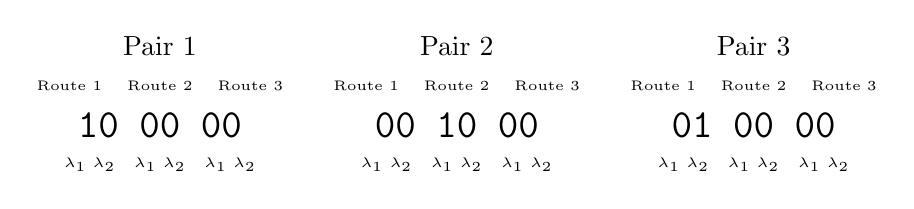
\begin{tikzpicture}[ every node/.style={align=center}]
    % First tuple
    \node at (0,1) {Pair 1};
    \node at (0,0.5) {\tiny Route 1 \quad Route 2 \quad Route 3};
    \node at (0,0) {\Large \texttt{10 00 00}};
    \node at (0,-0.5) {\tiny $\lambda_1 \ \lambda_2 \quad \lambda_1 \ \lambda_2 \quad \lambda_1 \ \lambda_2$};

    % Second tuple
    \node at (3.77,1) {Pair 2};
    \node at (3.77,0.5) {\tiny Route 1 \quad Route 2 \quad Route 3};
    \node at (3.77,0) {\Large \texttt{00 10 00}};
    \node at (3.77,-0.5) {\tiny $\lambda_1 \ \lambda_2 \quad \lambda_1 \ \lambda_2 \quad \lambda_1 \ \lambda_2$};

    % Third tuple
    \node at (7.54,1) {Pair 3};
    \node at (7.54,0.5) {\tiny Route 1 \quad Route 2 \quad Route 3};
    \node at (7.54,0) {\Large \texttt{01 00 00}};
    \node at (7.54,-0.5) {\tiny $\lambda_1 \ \lambda_2 \quad \lambda_1 \ \lambda_2 \quad \lambda_1 \ \lambda_2$};
\end{tikzpicture}
\caption{The bitstring representing a valid solution for an RWA instance where ${P} = 3, N = 3, {\Lambda} = 2$.
	%The bitstring is divided into three sub-bitstrings; each has $3 \times 2$ bits.
	%Each bit represent a selection of unique lightpath the corresponding source-destination pair.
}
\label{fig:bitstring}
\end{figure}

The mixer Hamiltonian that preserves the feasible solution subspace is \begin{align}
	\hat{H}_{m} &= \sum_{i = 1}^{{P}}
	\sum_{j = 1}^{N \times {\Lambda}}
	(\hat{X}_{i,j}\hat{X}_{i, j+1}+\hat{Y}_{i,j}\hat{Y}_{i, j+1}) .
\end{align}
\end{frame}

\begin{frame}{Formulation}{Two-steps scheme}
    \begin{itemize}
\item This amount of qubit may be unpractical when the scheme is applied on a utility scale.
\item The two-steps scheme is as follows:\begin{enumerate}
	\item Reduce the RWA problem into RA problem by letting the number of available wavelength, ${\Lambda} = 1$.
	\item Use the formulation to obtain the route for each source-destination node pair.
	\item Reintroduce the original number of available wavelength and let the route option be the ones obtained from the WA step.
\end{enumerate}
\item The two-step scheme reduces the number of qubits usage from ${P} \times N \times {\Lambda}$ to $\max(
{P} \times N, {P}  \times {\Lambda}
)$.
    
    \end{itemize}
\end{frame}

\begin{frame}{Numerical Results}{Classical simulation setup}
    % \item Results produced using classical simulation of QAOA in Qiskit
    % \item Simulation limited to $\leq 27$ qubits on local hardware
    % \begin{itemize}
    %     \item $(|V|=10, |E|=22)$
    %     \item $(|V|=20, |E|=42)$
    % \end{itemize}
    % Parameters varied:
    \begin{itemize}
        \item Number of requests: $2$ to $10$
        \item Number of alternate routes: $1$ to $10$
        \item Number of wavelengths: $1$ to $\abs{P}$
        \item Circuit depths $1$ to $4$
        \item Two network topologies
        \item Result compared to the $k$ shortest paths first-fit
    \end{itemize}
    % \item 142 RWA instances, depths $p=1$ to $p=4$
    % \item Baseline: $k$-shortest-path first-fit (k-SPFF)
    % \item Two random network topologies:
\begin{figure}[!htbp]
	\centering
	\begin{subfigure}{0.4\textwidth}
	\includegraphics[width=\textwidth]{pictures/plots/10.pdf}
	\caption{\scriptsize$\abs{V} = 10$ nodes and $\abs{E} = 22$ links. (Small)}
	\end{subfigure}
	\quad
	\begin{subfigure}{0.4\textwidth}
	\includegraphics[width=\textwidth]{pictures/plots/20.pdf}
	\caption{\scriptsize$\abs{V} = 20$ nodes and $\abs{E} = 42$ links. (Large)}
	\end{subfigure}
	\label{fig:toynetworks}
\end{figure}
%
% \begin{figure}[!htbp]
% 	\centering
% 	\begin{subfigure}{0.49\textwidth}
% 	\includegraphics[width=\textwidth]{pictures/plots/topology/route_freq_small.pdf}
% 	\caption{Small}
% 	\end{subfigure}
% 	\begin{subfigure}{0.49\textwidth}
% 	\includegraphics[width=\textwidth]{pictures/plots/topology/route_freq_large.pdf}
% 	\caption{Large}
% 	\end{subfigure}
% 	\caption{The frequency of the length of route (number of links) in each network topology}
% 	\label{fig:toynetworksroutefreq}
% \end{figure}

\end{frame}


\begin{frame}{Numerical Results: Performance}
\begin{itemize}
    \item Blocking ratio:
    \begin{itemize}
        \item At circuit depth $=1$: 20.7\% vs. 6\% ($k$-SPFF)
        \item At circuit depth $=4$: reduced to 18.0\%
    \end{itemize}
    \item Wavelength usage:
    \begin{itemize}
        \item QAOA (depth 1): 82.4\% vs. 86.9\% ($k$-SPFF)
        \item At depth 4: 79.6\%
    \end{itemize}
    % \item Runtime: QAOA simulation $\gg$ SPFF (exponential scaling)
    % \item Underperformance linked to barren plateau phenomenon \cite{grant2019-barren-plateu, McClean2018-barren-plateu, Cunningham2025-vqc-vqe-barren-plateu-taxonomy-literature-review}
\end{itemize}
\begin{figure}[H]
	\centering
	\begin{subfigure}{0.32\textwidth}
	\includegraphics[width=\textwidth]{pictures/plots/n_pairs/x-2-1-s.pdf}
	\caption{$N=2, {\Lambda} = 1$, small topology}
	\end{subfigure}
	\begin{subfigure}{0.32\textwidth}
	\includegraphics[width=\textwidth]{pictures/plots/n_pairs/x-1-2-m.pdf}
	\caption{$N=1, {\Lambda} = 3$, large topology}
	\label{pairb}
	\end{subfigure}
	\begin{subfigure}{0.32\textwidth}
	\includegraphics[width=\textwidth]{pictures/plots/n_pairs/x-1-3-m.pdf}
	\caption{$N=1, {\Lambda} = 3$, large topology}
	\label{pairc}
	\end{subfigure}
\caption{\scriptsize The blocking ratio and number of wavelength used.
\protect\reddashed is circuit depth $1$,
\protect\peachdashed is $2$,
\protect\pinkdashed is $3$,
\protect\skydashed is $4$, and
\protect\blackline is k-SPFF.
\label{fig:pairs}
}
\end{figure}

% \includegraphics[width=0.9\textwidth]{pictures/plotfigs/runtime.pdf}
\end{frame}


\begin{frame}{Numerical Results}{Effect of the modified cost function}
% \begin{itemize}
    % \item Original cost function: $ f(\mathbf{x}) = f_{\text{collision}} + f_{\text{wavelength}} $
    % \item Observation: wavelength penalty biases towards fewer wavelengths, ↑ blocking
    \textbf{Modification:} set $f_{\text{wavelength}} =0$. \\
    \textbf{Blocking ratio:} $\downarrow$ by $\sim$3.25\%, \textbf{Wavelength usage:} $\uparrow$ by $\sim$17\%\\
    \textbf{Top rows:} before cost function modification, \textbf{bottom row:} after
    % \item QAOA still underperforms baseline but trade-off becomes clearer
% \end{itemize}
    \begin{figure}[H]
\centering
\begin{subfigure}{0.32\textwidth}
	\includegraphics[width=\textwidth]{pictures/plots/n_pairs/x-1-2-s.pdf}
	% \caption{$N=1, \abs{\Lambda} = 2$, small topology}
\end{subfigure}
\begin{subfigure}{0.32\textwidth}
	\includegraphics[width=\textwidth]{pictures/plots/n_pairs/x-1-3-s.pdf}
	% \caption{$N=1, \abs{\Lambda} = 3$, small topology}
\end{subfigure}
\begin{subfigure}{0.32\textwidth}
	\includegraphics[width=\textwidth]{pictures/plots/n_pairs/x-2-2-s.pdf}
	% \caption{$N=2, \abs{\Lambda} = 2$, small topology}
\end{subfigure}
% \caption{Before}
	\label{fig:pairs_before}
\end{figure}

\begin{figure}[H]
	\centering
\begin{subfigure}{0.32\textwidth}
	\includegraphics[width=\textwidth]{pictures/plots/n_pairs/cc/x-1-2-s.pdf}
	\caption{\scriptsize $N=1, \abs{\Lambda} = 2$, small topology}
\end{subfigure}
\begin{subfigure}{0.32\textwidth}
	\includegraphics[width=\textwidth]{pictures/plots/n_pairs/cc/x-1-3-s.pdf}
	\caption{\scriptsize $N=1, \abs{\Lambda} = 3$, small topology}
\end{subfigure}
\begin{subfigure}{0.32\textwidth}
	\includegraphics[width=\textwidth]{pictures/plots/n_pairs/cc/x-2-2-s.pdf}
	\caption{\scriptsize$N=2, \abs{\Lambda} = 2$, small topology}
\end{subfigure}
% \caption{The blocking probability and number of wavelength used.
% \protect\reddashed represents $p=1$
% \protect\peachdashed represents $p=2$
% \protect\pinkdashed represents $p=3$
% \protect\skydashed represents $p=4$
% \protect\blackline represents SPFF
% }
% \caption{\scriptsize After}
\label{fig:cc_pairs}
\end{figure}

\end{frame}

\begin{frame}{Quality of Solutions: Distribution Analysis}
\begin{itemize}
    % \item QAOA produces a \textbf{distribution} over feasible states.
    \item Many sampled solutions are low-quality $\Rightarrow$ expected performance pulled down.
    \item Occasionally samples high-quality solutions (better than heuristic).
    % \item Probability of obtaining a “good” solution decreases with problem size.
    \item For small instances ($<20$ qubits), $\sim$10 measurement shots are sufficient to reach $>95\%$ confidence of finding a better solution.
\end{itemize}
\begin{figure}[H]
\centering
\begin{minipage}{.48\textwidth}
  \centering
	\includegraphics[width=\textwidth]{pictures/plots/prob/prob.pdf}
  % \captionof{figure}{The probability that the measured state will have lower blocking ratio when compared to the k-SPFF algorithm.}
	\label{fig:probprob}
\end{minipage}%
\hfill
\begin{minipage}{.48\textwidth}
  \centering
  \includegraphics[width=\textwidth]{pictures/plots/prob/num.pdf}
  % \captionof{figure}{The number of measurements required to measure a state with lower blocking ratio when compared to the k-SPFF algorithm 95\% of the time.}
	\label{fig:probnum}
\end{minipage}
\end{figure}


\end{frame}


\begin{frame}{Numerical Results: Two-steps scheme}
\begin{itemize}
        \item Joint formulation $\Rightarrow$ up to 20\% lower blocking
        \item Also uses fewer wavelengths than two-step scheme
        \item Confirms benefit of joint optimisation
\end{itemize}
\begin{figure}[!htbp]
\centering
\begin{subfigure}{0.49\textwidth}
\includegraphics[width=\textwidth]{pictures/plots/rawa/n_pairs/x-2-2-s.pdf}
	\caption{$\abs{P}=2, \abs{\Lambda} = 2$, small topology}
\end{subfigure}
\begin{subfigure}{0.49\textwidth}
\includegraphics[width=\textwidth]{pictures/plots/rawa/n_pairs/x-2-3-s.pdf}
	\caption{$\abs{P}=2, \abs{\Lambda} = 3$, small topology}
\end{subfigure}
\caption{%The blocking probability and number of wavelength used.
\protect\reddashed is the joint RWA formulation, and 
\protect\blackdashed is the two-steps formulation.
}
\label{fig:rawa}
\end{figure}

\end{frame}

\begin{frame}{Conclusion}
\begin{itemize}
    \item I proposed QAOA formulation for the joint RWA problem.
    \item The encoding uses one-hot constraints and a tailored mixer to guarantee feasibility.
    \item The joint formulation outperforms the two-step scheme.
    \item At small scales ($\leq 27$ qubits), QAOA underperforms classical heuristics in blocking.
\item Smarter cost-function shaping and adaptive mixers may improve performance.

\item Larger quantum hardware ($> 27$ qubits) will be needed to test the formulation at meaningful scales.
    \end{itemize}
\end{frame}

\begin{frame}[allowframebreaks]
\printbibliography
\end{frame}
\begin{frame}{Appendix}{Length of routes selected as alternate routes}
\begin{figure}[!htbp]
	\centering
	\begin{subfigure}{0.49\textwidth}
	\includegraphics[width=\textwidth]{pictures/plots/topology/route_freq_small.pdf}
	\caption{Small}
	\end{subfigure}
	\begin{subfigure}{0.49\textwidth}
	\includegraphics[width=\textwidth]{pictures/plots/topology/route_freq_large.pdf}
	\caption{Large}
	\end{subfigure}
	\caption{The frequency of the length of route (number of links) in each network topology}
	\label{fig:toynetworksroutefreq}
\end{figure}

\end{frame}

\begin{frame}{Appendix}{Expected cost at each iteration of the optimisation process}
\begin{figure}[H]
\centering
\begin{subfigure}{0.49\textwidth}
	\includegraphics[width=\textwidth]{pictures/plots/nit/9-1-3-s.pdf}
	\caption{$\abs{P}=9, N=1, \abs{\Lambda} = 3$, small topology}
\end{subfigure}
\begin{subfigure}{0.49\textwidth}
	\includegraphics[width=\textwidth]{pictures/plots/nit/6-2-2-s.pdf}
	\caption{$ \abs{P}=6, N=2, \abs{\Lambda} = 2$, small topology}
\end{subfigure}
\caption{The average cost of the solution at each iteration of QAOA.}
	\label{fig:nit}
\end{figure}


\end{frame}
\begin{frame}{Appendix}{Runtime}

\begin{figure}[H]
  \begin{center}
	\includegraphics[width=0.8\textwidth]{pictures/plots/time/time.pdf}
  \end{center}
	\caption{
	Runtime of the simulation at different problem size (quantified by the number of bits needed for the formulation).
      }
	\label{fig:runtime}
\end{figure}

\end{frame}

\end{document}

